\begin{solution}
\begin{enumerate}
\item {[10 points]} We have that
\begin{eqnarray*}
   \norm{g-g_N}^2 &=& \left( g-g_N, g-g_N\right) \\[0.5em]
 &=& \left( g - \sum_{n=1}^N \alpha_n \psi_n,
                           g - \sum_{m=1}^N \alpha_m \psi_m\right) \\[0.5em]
 &=& \left( g - \sum_{n=1}^N \alpha_n \psi_n, g\right) 
              -\sum_{m=1}^N \alpha_m \left( g - \sum_{n=1}^N \alpha_n \psi_n,   \psi_m\right) \\[0.5em]
 &=& \left(g,g\right) - \sum_{n=1}^N \alpha_n\left( \psi_n, g\right) 
              - \sum_{m=1}^N \alpha_m\left( g,   \psi_m\right) 
           +  \sum_{m=1}^N \alpha_m \sum_{n=1}^N \alpha_n (\psi_n, \psi_m) \\[0.5em]
 &=& (g,g) - \sum_{n=1}^N \alpha_n (\psi_n, g) 
           - \sum_{m=1}^N \alpha_m (g,\psi_m)
           + \sum_{n=1}^N \alpha_n^2  (\psi_n, \psi_n)\\[0.5em]
 &=& (g,g) - \sum_{n=1}^N \alpha_n (\psi_n, g) 
           - \sum_{m=1}^N \alpha_m (g,\psi_m)
           + \sum_{n=1}^N \alpha_n^2\\[0.5em]
 &=& (g,g) - \sum_{n=1}^N \alpha_n^2  
           - \sum_{m=1}^N \alpha_m^2 
           + \sum_{n=1}^N \alpha_n^2 \\[0.5em]
 &=& (g,g) - \sum_{n=1}^N \alpha_n^2 \\[0.5em]
 &=& \norm{g}^2 - \sum_{n=1}^N \alpha_n^2,
\end{eqnarray*}
where at each equal sign we have used:
(1) the definition of the norm $\norm{\cdot}$;
(2) the definition of $g_N$;
(3) linearity of the inner product in the second argument;
(4) linearity of the inner product in the first argument;
(5) the fact that $(\psi_n,\psi_m) = 0$ if $n\ne m$, for $m,n=1,2,\ldots,N$, since $\left\{\psi_1,\ldots,\psi_N\right\}$ is orthonormal with respect to the inner product $(\cdot,\cdot)$;
(6) the fact that $(\psi_n,\psi_n) = 1$, for $n=1,2,\ldots,N$, since $\left\{\psi_1,\ldots,\psi_N\right\}$ is orthonormal with respect to the inner product $(\cdot,\cdot)$;
(7) the fact that $(g,\psi_n) = (\psi_n,g) = \alpha_n$;
(8) algebra;
(9) the definition of the norm $\norm{\cdot}$.
\\
\item {[7 points]} From part (a) it follows that
\[
\norm{f-f_N}^2 = \norm{f}^2 - \sum_{n=1}^N c_n^2,
\]
where
\[
c_n={\sqrt{2} \over n\pi}\left(1-\left(-1\right)^n\right).
\]
Moreover,
\[
\norm{f}^2=\int_0^1\left(f(x)\right)^2\,dx=\int_0^11^2\,dx=\left[x\right]_0^1=1
\]
and so
\[
\norm{f-f_N}^2 = 1 - \sum_{n=1}^N c_n^2.
\]
The requested plot and the code used to produce it is shown in part (c).
\\
\item {[8 points]} From part (a) it follows that
\[
\norm{u-u_N}^2 = \norm{u}^2 - \sum_{n=1}^N d_n^2,
\]
where
\[
d_n={\sqrt{2} \over n^3\pi^3}\left(1-\left(-1\right)^n\right).
\]
Moreover,
\begin{eqnarray*}
\norm{u}^2&=&\int_0^1\left(u(x)\right)^2\,dx
\\
&=&\int_0^1{1\over 4}x^2\left(1-x\right)^2\,dx
\\
&=&{1\over 4}\int_0^1x^2-2x^3+x^4\,dx
\\
&=&{1\over 4}\left[{1\over 3}x^3-{1\over 2}x^4+{1\over 5}x^5\right]_0^1
\\
&=&{1\over 4}\left({1\over 3}-{1\over 2}+{1\over 5}\right)
\\
&=&{1\over 4}\left({10\over 30}-{15\over 30}+{6\over 30}\right)
\\
&=&{1\over 4}{1\over 30}
\\
&=&{1\over 120}
\end{eqnarray*}
and so
\[
\norm{u-u_N}^2 = {1\over 120} - \sum_{n=1}^N d_n^2.
\]

The requested plot is shown below. 

\begin{center}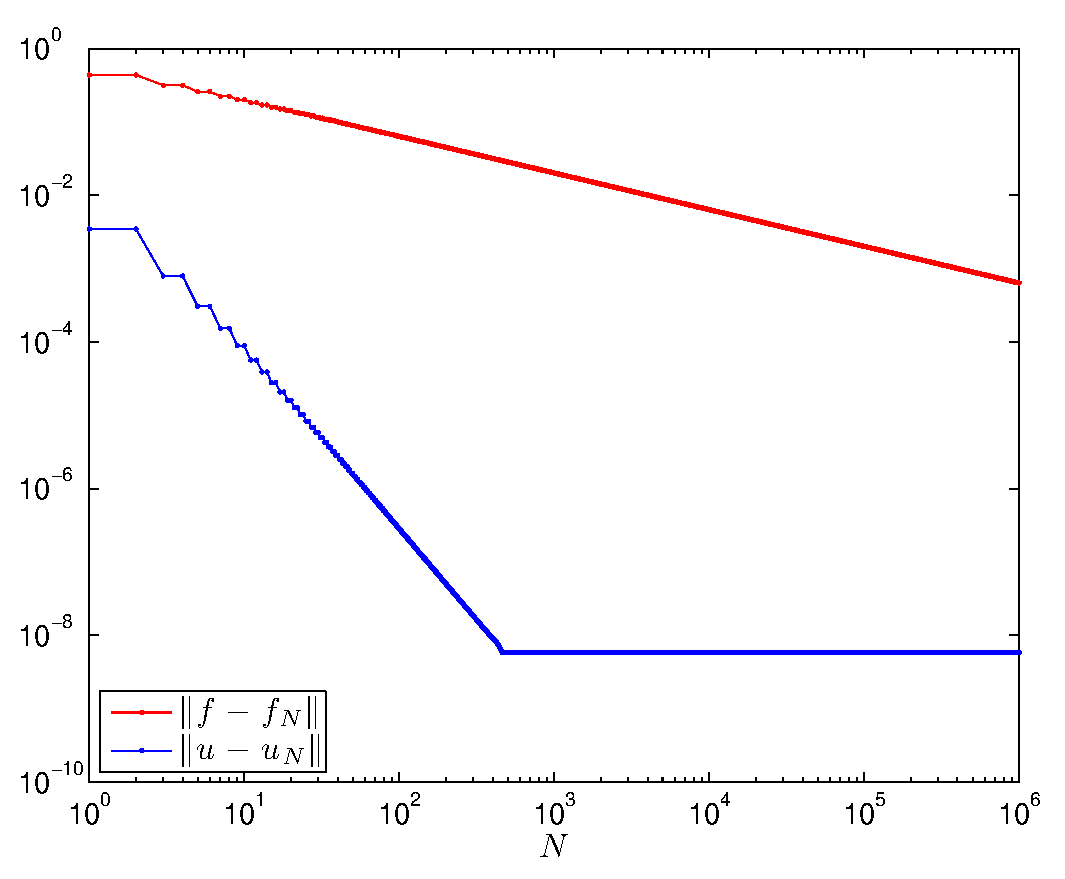
\includegraphics[scale=0.7]{fourerr}\end{center}
\end{enumerate}

The code that produced the plot is shown below.

\lstinputlisting{HW25bc.m}

\end{solution}
